\section{Introduction}
\label{sec:intro}
In this project, we aim to develop a model capable of classifying paintings according to their artistic style. Following the approach proposed in \cite{imran2023artistic}, our model consists of two components: a deep neural network (DNN) classifier and a shallow neural network (SNN).

At the first stage, each input image is divided into five distinct patches:
top-left, top-right, bottom-left, bottom-right, and center (as illustrated in
Figure 2). The DNN independently classifies each of these five patches. In the
second stage, the SNN functions as a decision-maker: it takes the probability
distributions generated by the DNN for the five patches as input and produces
the final classification result. According to \cite{imran2023artistic}, this
two-stage architecture helps reduce error accumulation by training the two
stages separately.

Our project consists of two main parts:
\begin{itemize}
  \item \textbf{Architecture implementation and validation:} Implement the architecture mentioned in \cite{imran2023artistic} (since there is no open-source code repo), and prove its effectiveness by ablation study.
  \item \textbf{Adaptive refinement and optimization:} To further explore and gain insights, we investigate how certain design choices affect model accuracy, including:
        \begin{itemize}
          \item \textbf{Selection of the fifth patch}: Instead of always choosing the center region as the fifth patch, we experiment with alternative strategies such as using a downsampled version of the entire image or extracting a region that contains the main semantic content.
          \item \textbf{Architectural variations}: Beyond the simple five-patch individual classification scheme, we explore more complex hierarchical architectures. We evaluate their performance and analyze the results to understand how these modifications influence classification accuracy.
        \end{itemize}
\end{itemize}
\begin{figure}[h]

  \centering
  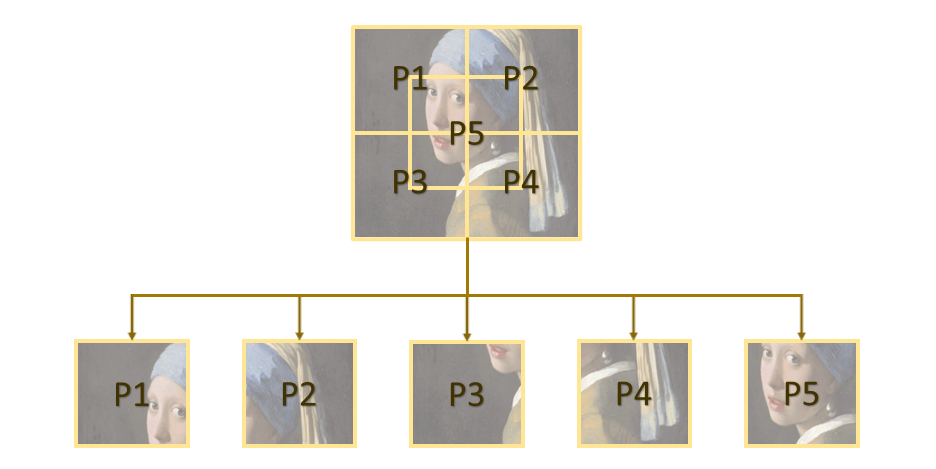
\includegraphics[scale=1,keepaspectratio,width=.5\textwidth]{patch.png}
  \caption{Patch division}
  \label{fig:main_pipeline}
\end{figure}